% Copyright 2021 Thomas Ascher
% SPDX-License-Identifier: CC-BY-SA-4.0

\documentclass[a4paper,parskip=half]{scrartcl}

\usepackage[T1]{fontenc}
\usepackage[ngerman]{babel}
\usepackage{csquotes}
\usepackage[regular,condensed,sfdefault]{roboto}
\usepackage{graphicx}
\usepackage{chemformula}
\usepackage{amsmath,amsfonts,amssymb}
\usepackage[italic,symbolgreek]{mathastext}
\usepackage[backend=biber]{biblatex}
\usepackage[hidelinks,pdfencoding=auto,
  pdfauthor={Thomas Ascher},
  pdfusetitle,
  pdfkeywords={Bier,Refraktometer,Alkoholmessung,Terrill,Novotný}]{hyperref}
\usepackage{microtype}

\addto\extrasngerman{
\def\figureautorefname{Abb.}
}

\addto\captionsngerman{
\renewcommand{\figurename}{Abb.}
}

\title{Alkoholmessung mit dem Refraktometer}
\author{Thomas Ascher}
\date{14. August 2021, \href{http://creativecommons.org/licenses/by-sa/4.0/}{CC BY-SA 4.0}}

\addbibresource{refraktometer.bib}

\newcommand{\bxi}{\mathit{B}_i}
\newcommand{\bxic}{\mathit{Bc}_i}
\newcommand{\bxf}{\mathit{B}_f}
\newcommand{\bxfc}{\mathit{Bc}_f}
\newcommand{\sg}{\mathit{SG}}
\newcommand{\fg}{\mathit{FG}}
\newcommand{\abv}{\mathit{ABV}}
\newcommand{\abw}{\mathit{ABW}}
\newcommand{\oex}{\mathit{OE}}
\newcommand{\aex}{\mathit{AE}}
\newcommand{\rex}{\mathit{RE}}
\newcommand{\wcf}{\mathit{WCF}}
\newcommand{\adf}{\mathit{ADF}}
\newcommand{\rdf}{\mathit{RDF}}


\begin{document}
\maketitle

\section*{Einleitung}

stabiler, schnellere Probenkühlung,
\autocite{Terrill2013}

nicht besser als Hydrometer
\autocite{Terrill2011}


0,6 \% Fehler ungenauer als andere methoden, schnelle prüfung,
hohe Probenanzahl. Alle 10 Jahre neu
\autocite{Bettner1969}

1843 Studien zwischen RI und Alkoholgehalt
Lich brechung Refraktion
zweite dichter adteilung des Sichtsfeldes in Hell Dunkel Critical Ray,

\autocite{Gamer1959}

\section*{Messprinzip}

The International Commission for Uniform Methods of Sugar Analysis  Ltd. (ICUMSA) -> Umrechnung.

Je dichter Flüssigkeit, desto langsamer licht durch,, Prisma misst, , dichter stärkere Brechung.  R = Verhältnis von licht im
Vakuum zu licht in der Flüssigkeit.
Kalibriert auf bestimmte Lösung bei bestimmter Temperatur,
Brix 20 °C
\autocite{Bonham2001}


maß wie licht abgebremst wird durch probe,
misst brechungsindex, optisches messen, licht durch probe, abgelenkt
prisma auf linse projiziert auf Fadennetz mit Skala, ansicht in Okular
Farblichen farbloser Bereich
auf verschiedene anwendungen kalibrierte skala, z.b. Brix.
1Bx = 1g Saccharose (Haushaltszucker) auf 99g Wasser. ähnlich zu plato
gleich behandelt
digital refraktometer -> licht intefferenz, verschiedene skalen, messbereich
ATC -> bimetall streifen, ATC nicht für Würze geeignet, falsche Korrektur
nicht für jede Substanz geeiget, ATC 10-30°C
\autocite{Terrill2013}

ATC verursacht fehler weil auf Zucker geeicht
\autocite{Terrill2010}

SG skala ungenau
\autocite{Terrill2011}

andere Temperatur verursacht verzerrung
ASBC refractometry protocols, Kurfenanpassung pro würze
\autocite{Bonham2001}

ATC nicht
für alle Probe geeignet. -> sugar Water
\autocite{Depalma2017}

Refi misst index Lichtbrechung
mehr alk -> höhere RI
Dichte Temperatur abhängig, 20°C
\autocite{Gossett2012}

Licht wechselt Richtung, wenn optisch weniger dichtes zu dichteres Medium
RI maß für Brechung

\autocite{Spedding2016}

analog refractometer performed as well as the bench-top, digital refractometer
problems develop that limit precision.  For example, some dark and turbid samples will give rather fuzzy lines of demarcation when one tries to read the analog scale.  Often this fuzziness gets worse with time as the sample sits on the glass slide, presumably as solids settle or gas bubbles form.  The fuzziness of the demarcation line serves as a kind of warning to the user. 
mehrfache Messung bei digitalen
\autocite{Gossett2012a}

\section*{Exkurs Hydrometer}

Auftrieb, = gewicht der verdrängten flüssigkeit, sinkt weiter
ein bei weniger dichten Würze.
100 bis 200 ml Probe
co2 in Lösung beeinflusst den Messwert um circa 0.3 P
Refraktometer weniger einfluss durch co2
Messung fg zu niedrig wegen Alkoholfehler
\autocite{Novotny2017}

Dichtemessung, geringere Dichte sinkt weiter ein, 20°C kalibriert.
masse \%, Zucker lösung, saccarose, von oben oder unten lesen je
nach angabe -> Flüssigkeitsmeniskus.
Würze bzw. Probe gut durchmischen. kein Wasser am Hydrometer trocken
sein, nicht zu tief eintauchen um Würze Anhaftung zu vermeiden
Korrektur notwenig bei anderer Temp -> Dichteänderung
Umrechnung zwischen dichte und Extraktgehalt erfolgt über Plato Tabelle
Alkoholfehler Messabweichung.
Balling Faktor 0.81
\autocite{Kunze2004}

Alkoholmessung bei 20°C Ethylalkohol Ethanol im Bier
Volumen Abhängig von Temperatur
0.3 \% Toleranz in den USA
SG = Einheitenlos, realtiv zu std Substanz z.B. Wasser in 20 °C
AE = änderung der Dichte, verfälscht durch Alkohol
RE = maß des verbleibenden Zuckers + Protein und Sonstige
g Extrakt / 100g Bier = Plato.
RDF real degree of fermentation
Hydrometer Prinzip Auftrieb, Messfehler durch Solids + Gase
Temp Kompensation notwendig,
SG oder Plato. 
\autocite{Spedding2016}

\autocite{Brueckelmeier2018}

Sie wird in der Praxis mit Saccharometern durchgeführt, die auf dem Prinzip
der Aräometer beruhen. Nachdem ursprünglich die Saccharometer nach Balling
anhand einer Rohrzuckerlösung geeicht waren, ist an die Stelle der Ballings-
chen Tabelle die der Normaleichungskommission (PLATO) getreten [1039]. Die
Brauereisaccharometer sind als Thermosaccharometer ausgebildet, die die Wer-
te bei 20 8C angeben. Anhand einer Reduktionsskala werden bei Temperaturen
über 20 8C Korrekturwerte hinzugezählt, bei Temperaturen unter 20 8C dagegen
abgezogen. Die Genauigkeit der Saccharometeranzeige ist nur bei geeichten
Spindeln, die am besten in bestimmte Messbereiche eingeteilt sind (0–5, 5–10,
10–15, 15–20\%), zufriedenstellend.
Bei genauen Messungen, wie sie z. B. bei Sudhausabnahmen erforderlich
sind, muss eine Extraktbestimmung im Laboratorium, mittels Pyknometer oder
Biegeschwinger vorgenommen werden. Die zur Aufnahme der Würzeprobe die-
nenden Gefäße müssen trocken sein.

Der Extraktgehalt ist in Gewichtsprozenten angegeben, d. h. eine 12%ige
Würze enthält in 100 g: 12 g Extrakt und 88 g Wasser.
Um genaue Ergebnisse zu erhalten und Ablesefehler zu vermeiden, sind fol-
gende Punkte zu beachten:
a) das Saccharometer muss rein und trocken sein; es soll ungefähr jene Tem-
peratur haben wie die zu messende Flüssigkeit;
b) das Messgefäß muss rein und mit der zu spindelnden Flüssigkeit vorgespült
sein;
c) das Messgefäß muss in der Waage stehen; dies wird auch durch eine Kar-
danaufhängung bewirkt;
d) das Messgefäß muss so weit sein, dass das Saccharometer, ohne zu großen
Spielraum, bequem Platz findet;
e) vor dem Ablesen wird das Saccharometer mehrmals rasch eingetaucht und
wieder herausgezogen, um anhaftende Gasblasen zu entfernen;
f) die Ablesung des Saccharometers erfolgt am oberen Ende des sich an der
Spindel ausbildenden Meniskus der Flüssigkeit, sofern dies nicht eigens an-
ders vermerkt ist.
g) Bei Abkühlen der Würze wird durch Abdecken eine Verdunstung vermieden;
vor der Spindelung ist die abgekühlte Flüssigkeit durch mehrmaliges
Stürzen zu mischen.
Es ist von entscheidender Bedeutung, dass die Entnahme der Würzeprobe zur
Extraktermittlung und die Erfassung der Würzemenge in der Pfanne zur glei-
chen Zeit vorgenommen werden. Es besteht sonst die Gefahr, dass durch ein
weiteres Verdampfen von Wasser, z. B. bei stark ziehenden Pfannen, eine Verfäl-
schung der Ergebnisse der Ausbeuteermittlung eintritt.
Bei modernen Würzekochsystemen ist die Entnahme einer repräsentativen
Würzeprobe schwierig; es können sich, z. B. bei geöffneter Pfannentür Konzent-
rationsunterschiede durch Verdunstung oder generell Probleme durch Inhomo-
genitäten ergeben.
\autocite{Narziss2009}

\section*{Kalibrierung und Justierung}

2 punkt 20°C, 0 Stellung jeden Tag, Wasser 0° Bx, Referenzlösung herstellen,
mit kalibrierter Feinwaage
\autocite{Terrill2013}

Kalibrierung bei Umgebungstemperatur.
\autocite{Bonham2001}

Deionisiertes Wasser und Kalibrierung auf 0, NIST standard
organisation
\autocite{Depalma2017}

Rene Fehler von 2 Brix.

Ein, zweipunkt, mehrpunkt
\autocite{Earl2015}

schlechte chinestischer herstellung
\autocite{Troester2012}

\section*{Würze-Korrekturfaktor}

\begin{equation}
\wcf = \frac{\bxi}{\mathit{OE}}
\end{equation}

\begin{equation}
\oex = \bxic = \frac{\bxi}{\wcf}
\end{equation}

1.04 nicht konstant, Proteine, Säuren und Salze Einwirkung
darauf.
\autocite{Roberts1950}

WCF = refrakto / hydro, 1.02-1.06, 1.04 guter Durchschnitt. Abhängig von Würze
Mehr adjunkte kleinerer Faktor
\autocite{Terrill2013}

Dichte Lösung Zucker nicht dichte Würze
RI 15 \% Maltose 1,3362, Succrose 1,3557 15.3, 
WCF = refrakto Bx  / Hydro in P
\autocite{Bonham2001}

\autocite{Weiss2016} 1.03

\section*{Messung durchführen}

einige Tropfen auf Refi, nicht heiß tropfen lassen, verschlossen auskühlen
\autocite{Terrill2013}

trocken und sauber
\autocite{Bonham2001}

Möglichst genau durchführen, 0.25 P in Hydrometer Fehler,
0.25 \% ABV Fehler
\autocite{Bonham2001}

Messfehler durch fehlende Temperaturkontrolle, ATC nicht
für alle Probe geeignet.
Kreuzkontaminierung durch schlecht gereinigte
\autocite{Depalma2017}

Schwebstoffe und Gas entfernen, gute Beleuchtung
\autocite{Gamer1959}

\section*{Korrelationsfunktionen zur Schätzung des scheinbaren Restextrakts}

Faktoren Anpassen
\autocite{Gamer1959}

durch alkoholfehler misst nicht AE, dnerer RI, Korrelation notwendig.
\autocite{Terrill2010a}

linearer zusammenhang zwischen Vergärungsgrad und Alkoholgehalt,
gleicher RI für verschiedene Probenzusammensetzung.
\autocite{Terrill2010}

Temperatur abhängig, 20°C
\autocite{Gossett2012}

\subsection*{Gardner (2000)}

% equations derived by Roberts & Stewart: 1
ausreichend genau für den Heimbereich
\autocite{Bonham2001}

\begin{equation}
\mathit{AE}=1,53 \cdot \bxf - 0,59 \cdot \bxic
\label{eq:gardner} 
\end{equation}

\subsection*{Bonham (2001)}

Standard \autocite{Terrill2010a}

Laut Gossett Bonham formel falsch angewendet Bx korrigiert.
Gemessen 10 Biere bei Stammwürze von 9 - 24 und bei Standard Formel Abweichungen
beim AE festgestellt von 0.1 - 2.2 Plato, keine Abweichung bei
58\% RDF (71\% ADF), mean = 1.3 °Plato
\autocite{Terrill2010a}

Quelle nicht bekannt, auch wenn korrekt insignifikante verbesserung
\autocite{Terrill2011}

\autocite{Bonham2001}

\begin{align}
\begin{split}
\fg &= 1,001843 - 0,002318474 \cdot \bxic - 0,000007775 \cdot \bxic^2 -
0,000000034 \cdot \bxic^3 \\
& \quad + 0,00574 \cdot \bxf +
0,00003344 \cdot \bxf^2 + 0,000000086 \cdot \bxf^3
\end{split} \label{eq:bonham} 
\end{align}

\subsection*{Terrill (2011)}

12 Biere, 8 kommzerielle Brauereien evaluiert, 88 \% des AE liegt innerhalb
von 0.5 °P
\autocite{Terrill2013}

OE: 9 - 24, AE: 1.8 - 5.6, ADF - 73 \% to 91 \%, 60 Messungen,
\autocite{Terrill2010}


Bonham Formel quelle nicht bekannt
50 \% RDF (61 \% ADF) Proben gemessen wurden aber verworfen, weil
Genauigkeit verschlechtert.
Abweichungen bein linearen besser als vereinfachte Kubische
ADFs from 73 \% to 91 \% Ergebnisse
\autocite{Terrill2011}

mean, std, max, <0.5°P
old: -0.4, 0.6, -2.1, 41 \%
new cubic: 0.2, 0.3, 1.2, 85 \%
new linear 0.03, 0.4, 1.0, 84 \%

\autocite{Terrill2011}


\begin{equation}
\fg = 1 - 0,00085683 \cdot \bxic + 0,0034941 \cdot \bxfc
\label{eq:terrilllinear} 
\end{equation}

\begin{align}
\begin{split}
\fg &= 1 - 0,0044993 \cdot \bxic + 0,011774 \cdot \bxfc + 0,00027581 \cdot \bxic^2 - 0,0012717 \cdot \bxfc^2 \\
& \quad  - 0,0000072800 \cdot \bxic^3  + 0,000063293 \cdot \bxfc^3
\end{split} \label{eq:terrillcubic} 
\end{align}

\subsection*{Gossett (2012)}

unzufrieden mit indirekter Messwert mit Umrechnung von
unbekannter Genauigkeit.
Auswirkung von Alkoholgehalt auf den Brix Messung.
Stochiometrisches Modell. 12 Biere im Vergleich mit
Hydrometer. Kochen Verdünnung.
\autocite{Gossett2012}

0.445 Brix (20°C) per \% ABW, 
Standardabweichung bei 0.1 Brix Genauigkeit  \%ABV of 0.115/0.353 = 0.33
und Ausschluss systematischer Messfehler.
\autocite{Gossett2012a}

Formeln
\autocite{Gossett2012b}

\begin{equation}
k = 0,445
\end{equation}

\begin{equation}
C = 100 \cdot \frac{\bxi - \bxf}{100 - 48,4 \cdot k - 0,582 \cdot \bxf}
\end{equation}

\begin{equation}
\abw = \frac{48,4 \cdot C}{100 - 0,582 \cdot C}
\label{eq:gossett} 
\end{equation}

Bonham zur FG Bestimmung.

12 Biere Mittlere Abweichung 0.1 ABV, Standardabweichung 0.4 ABV
model std dev 0.2 \%ABV. beo 0.1 brix auflösung

\autocite{Gossett2012c}

\begin{equation}
\aex = \bxic - \frac{\abw \cdot (2,0665 - 1,0665 \cdot \bxic / 100)}{0,8052}
\end{equation}

\subsection*{Novotný (2017)}

ABW, RE Formeln

Verglichen mit Terrill Formel 65-80 \% Vergärungsgrad genau,

Petr Kosin

3 Biere bei 11,6, 17, 22,9 OE, genauigkeit innerhlb von
0.26 °P, bei Hydrometer 0.15 °P abezogen wegen CO2
2 Tage besseres ergebnis als Terrill
\autocite{Novotny2017}

Vergleichwerte
\autocite{Novotny2017a}


\begin{equation} 
\fg = -0,002349 \cdot \bxic + 0,006276 \cdot \bxfc + 1
\label{eq:novotnylinear} 
\end{equation}

\begin{align}
\begin{split}
\fg &= 1,335 \cdot 10^{-5} \cdot \bxic^2 - 3,239 \cdot 10^{-5} \cdot \bxic \cdot \bxfc + 2,916 \cdot 10^{-5} \cdot \bxfc^2 \\
& \quad - 2,421 \cdot 10^{-3} \cdot \bxic + 6,219 \cdot 10^{-3} \cdot \bxfc + 1
\end{split} \label{eq:novotnyquadratic} 
\end{align}

\autoref{eq:novotnylinear}

%(\autoref{fig:groteblohm}) von 
%Grote \& Bohm \autocite{GroteBlohm2020}.

%\begin{figure}[h]
%\centering
%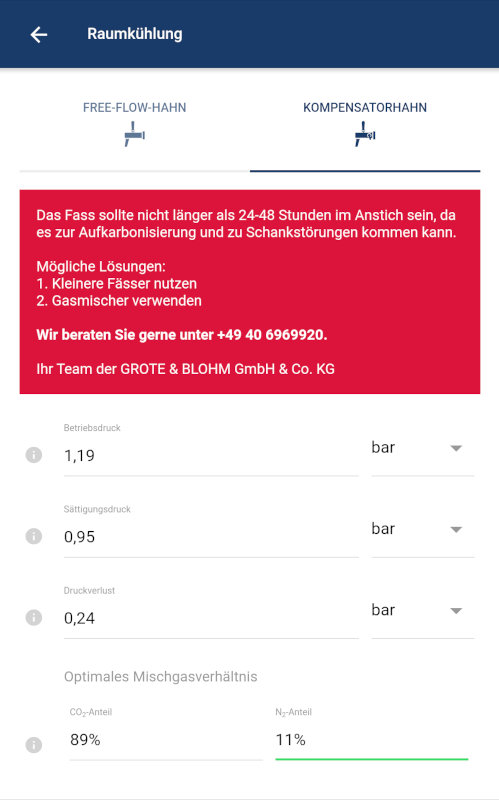
\includegraphics[width=4.8cm]{images/groteblohm.jpg}
%\caption{FOBB-APP}
%\label{fig:groteblohm}
%\end{figure}

\subsection*{Welche Korrelationsfunktion?}

Novotný
\href{https://brewfather.app}{Brewfather}
\href{https://www.brewersfriend.com/refractometer-calculator}{Brewer's Friend}

Terrill
„\href{https://braureka.de/berechnungen/refraktometer-korrektur/}{BräuReKa!}“
\href{https://www.maischemalzundmehr.de/index.php?inhaltmitte=toolsrefraktorechner}{Maische, Malz und Mehr} + Bonham
\href{https://mashcamp.shop/brauberechnungen}{MashCamp}

\href{http://www.brewrecipedeveloper.de}{Brew Recipe Developer}

Die Standardformel dagegen liefert entlang des gesamten Gärverlaufs gleichmäßig gute Werte, weicht aber in endvergorenen oder nahezu endvergorenen Proben weiter von den wahren Werten ab als die Terrill-Formel. D
\autocite{Weiss2016}

\section*{Berechnung des Alkoholgehalts}

Aus konsumierter Zuckermenge und der Balling Formel lässt sich

the following values must be known or
obtained: the present or apparent gravity of the beer, the real extract of the beer,
the specific gravity of the alcohol contained within the beer, and the original extract
of the wort (terms defined in Table 7.1). To help solve for these various terms, it is
noted that an arithmetic relationship exists between them through which Carl Ball-
ing first laid down the foundation for brewing calculations

\begin{equation}
\sg = \frac{P}{258,6 - \mathit{P} / 258,2 \cdot 227,1} + 1
\end{equation}

\begin{equation}
P = -205,347 \cdot \sg^2 + 668,72 \cdot \sg - 463,37
\end{equation}

\begin{equation}
\rex = 0,1948 \cdot \oex + 0,8052 \cdot \aex
\end{equation}

\begin{equation}
\abw = \frac{\oex - \rex}{2,0665 - 1.0665 \cdot \oex / 100}
\end{equation}

\begin{equation}
\abv = \frac{\abw \cdot \fg}{0,7907}
\end{equation}

\autocite{Spedding2016}

\begin{equation}
\adf = 100 \cdot \frac{\oex - \aex}{\oex}
\end{equation}

\setlength{\jot}{2mm}

\begin{equation}
\rdf = 100 \cdot \frac{\oex - \rex}{\oex} \cdot \frac{1}{1 - 0,005161 \cdot \rex}
\end{equation}

\autocite{Speers2015}

Lincoln equations
\autocite{Spedding2016}

Method \href{https://www.asbcnet.org}{American Society of Brewing Chemists (ASBC)} \href{https://www.mebak.org}{Mitteleuropäische Brautechnische Analysenkommission (MEBAK)}

\section*{Berechnungsbeispiel}

Linear

bxi = 12
bxf = 6
wcf = 1.04

Referenzimplementierung \url{https://aschet.github.io/refractometer/}


\begin{align*}
\bxi &= 12 \\
\bxf &= 6 \\
\wcf &= 1,04 \\
\oex = \bxic = \frac{12}{1.04} &= 11,54 \\
\bxfc = \frac{6}{1.04} &= 5,77 \\
\fg = 1 - 0,00085683 \cdot 11,54 + 0,0034941 \cdot 5,77 &= 1,010 \\
\aex = -205,347 \cdot 1,010^2 + 668,72 \cdot 1,010 - 463,37 &= 2,63 \\
\rex = 0,1948 \cdot 11,54 + 0,8052 \cdot 2,63 &= 4,37 \\
\abw = \frac{11,54 - 4,37}{2,0665 - 1,0665 \cdot 11,54 / 100} &= 3,69 \\
\abv = \frac{3,69 \cdot 1,010}{0,7907} &= 4,71
\end{align*}

\section*{Zusammenfassung}

\printbibliography[title=Quellen]

\end{document}